\section{Marco Teórico}

% \subsection{Climatología}

% Según las definiciones de la RAE

\subsection{Meteorología}

La RAE define a la meteorología como la ciencia que estudia los fenómenos atmosféricos. Esta se encarga, entre otras cosas, de crear modelos para la predicción del clima. Para crear dichos modelos, es necesaria la recolección de diversos datos.

Los datos meteorológicos que se requiere recabar para usos meteorológicos están definidos en la guía para los instrumentos meteorológicos y métodos de observación (conocida como la guía \textit{CIMO}), publicada por la Organización Meteorológica Mundial (\textit{WMO} en adelante) \cite{CIMO_2008}. Esta guía, establece una serie de criterios y estándares que deben ser utilizados para la definición, recolección y uso de los datos meteorológicos.

Entre los datos que es necesario recabar, podemos encontrar la temperatura. La cual es definida como una cantidad física que caracteriza el movimiento aleatorio de moléculas en un cuerpo físico. Para fines meteorológicos, se toma la temperatura media como punto de medición, y comúnmente se mide la temperatura del aire a diversas altitudes. Sin embargo, también son utilizadas otras temperaturas, como la de el suelo, la tierra y la temperatura de el agua marina. En el caso de la temperatura del aire, esta se define como la temperatura de un termómetro en un expuesto al aire pero cubierto de la luz directa del sol.

Otro de los datos importantes para la meteorología, es la presión atmosférica es definida por la WMO \cite{CIMO_2008} como la cantidad de presión ejercida por la atmósfera en un punto, en medida de fuerza por unidad de área. Además de la presión, la WMO también recomienda el calcular la tendencia de la presión. Esta es definida como la cantidad de cambio de presión en un lapso de 3 horas.

De la misma forma, la velocidad del viento es un dato requerido para el análisis meteorológico, el cual se define como un vector tridimensional de cantidad con variaciones pequeñas aleatorias, y caracterizado por fluctuaciones rápidas llamadas ráfagas. Generalmente se utiliza la representación polar del promedio de velocidad horizontal del viento, y su dirección como dato meteorológico \cite{CIMO_2008}.

La humedad específica es el radio entre la masa de vapor de agua y la masa de aire húmedo. en cambio, la humedad relativa es el radio entre el porcentaje de la presión observada del vapor y la saturación de la presión del vapor con respecto al agua a la misma temperatura y presión.

\subsection{Estación meteorológica}

Una estación meteorológica es un aparato que puede ser electrónico o analógico que posee sensores, generalmente estandarizados para la medición y toma de datos ambientales \cite{CIMO_2008}. Cabe notar que en el caso de las estaciones meteorológicas electrónicas, estas poseen un tiempo de \textit{enfriamiento} entre cada medición de un dato ambiental \cite{davis:6152C_6162C_SS}.

Debido al alcance físico de una estación meteorológica, se ha optado por realizar redes de estaciones. Entre estos tipos de redes, podemos encontrarnos con las redes meteorológicas urbanas, las cuales son una metodología de recolección de datos especialmente útil para ambientes de población urbanos con una densidad alta, que requiere de una cantidad considerable de sensores distribuidos . Muller \textit{et al} \cite{doi:10.1002/joc.3678} describen las redes meteorológicas urbanas como un elemento esencial para monitorear los procesos atmosféricos y para evaluar tanto el cambio climático a largo plazo como los eventos meteorológicos a corto plazo.

% \begin{figure}[ht!]
%    \centering
%    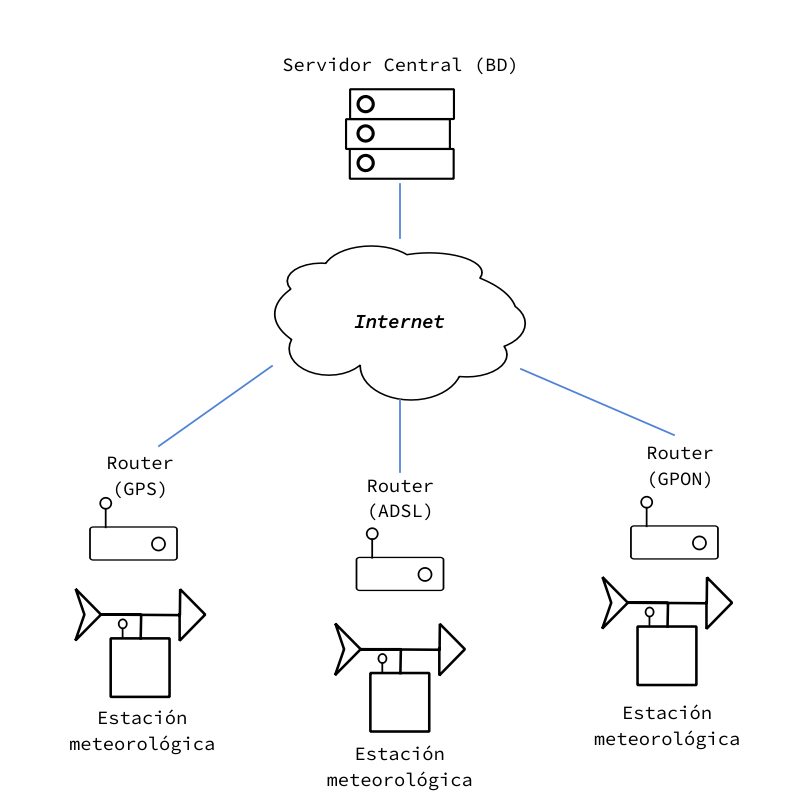
\includegraphics [ width = 0.8\textwidth ] {images/stations_arrangement.png}
%    % 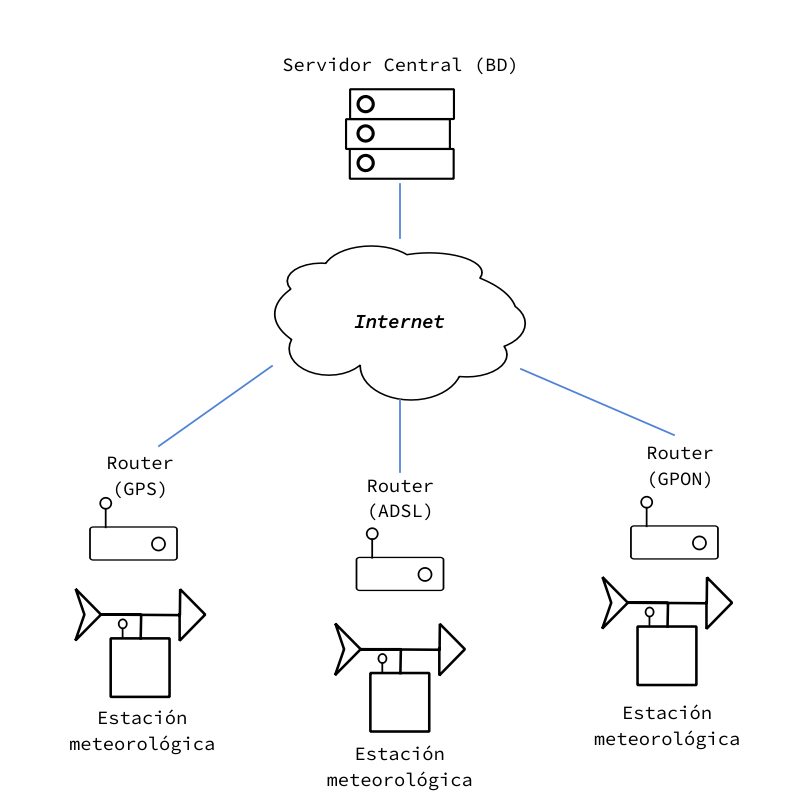
\includegraphics [ height = 160px ] {images/stations_arrangement.png}
%    \caption{Organización de las estaciones meteorológicas en el laboratorio CECATEV de la UACJ}
%    \label {fig:stations}
% \end{figure}


% \subsection{Transformada de ondícula}

% \cite{daubechies1990wavelet},

% \subsection{Métodos de compresión}

% La compresión de datos se realiza por medio de diversas

%    Ruido
%       Reducción de ruido
%       Normalización de temperatura por medio de Filtros
%    Fourier

